\subsection{Numerical Examples and Threshold Setting}\label{sec:aggregation:performance_model:numerical_examples}

Using the model we aim to calculate numerical examples to evaluate the performance of the system in different scenarios.
%In the following we analyse the performance of a system with two server groups.
%The analytical model and the simulation are described.
As parameters we study the load on the reference system $\rho_1$ and the load on the cooperating system $\rho_2$.
We consider the blocking probability of the reference system $p_{b_1}$ and the normalized received bandwidth of the reference system $E[X_{A_1}]/n_1$.
To validate our model and to get a first assessment, we analyse the performance of systems with equal thresholds and compare the analytic results with the results obtained from simulation and those of simple reference systems.
We consider the symmetric case with even load $\rho_1=\rho_2$ to investigate the impact of the offloading thresholds and to optimize them.
We then consider the asymmetric case to analyse the performance of systems with imbalanced load.
We conduct parameter studies to find system configurations where one of the systems can highly benefit from offloading, e.g. by being prioritized.
Finally we run simulations with different service time distributions to assess the system performance in more general cases.

\begin{figure}[tb]
	\centering
	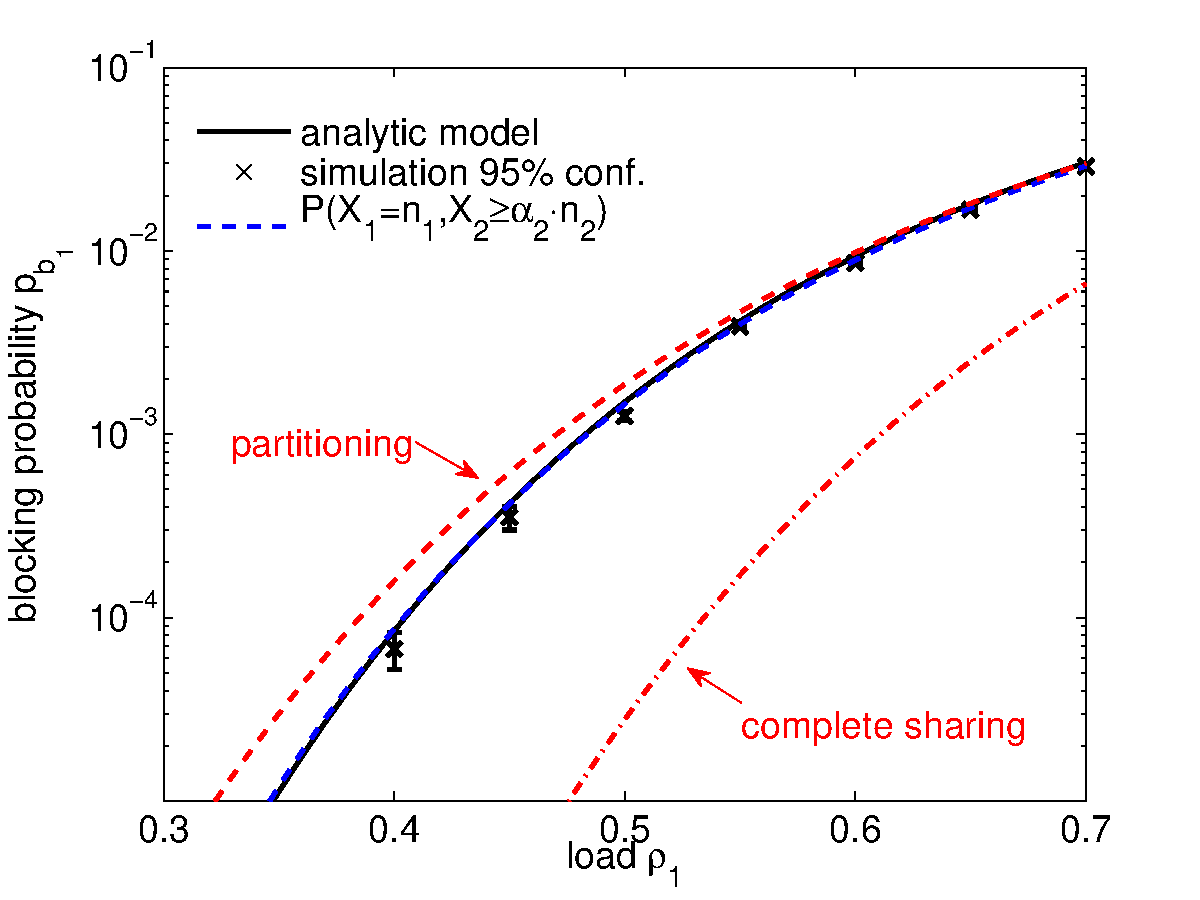
\includegraphics[width=0.5\textwidth]{aggregation/performance_model/figures/m2_n20_comp}
 	\caption{Blocking probability of two systems with equal load.}
 	\label{fig:m2_comp}
\end{figure}

Figure~\ref{fig:m2_comp} shows the blocking probability dependent on the system load of two server groups with equal arrival processes.
In this case the blocking probability is equal for both systems. Both systems have $n=20$ bandwidth fractions, and the thresholds are set to $\alpha=40\%$ and $\beta=80\%$.
The black line shows the result based on the analytic model for a composite system as described in Section~\ref{sec:analysis}.
The markers show the mean of 8 simulation runs with 95\% confidence intervals.
The blocking probability increases with the load on the system as expected.
The results of the simulation match the analytical model with high confidence.

For comparison the analytic result for the approximation $\tilde{p}_b$, for partitioning and for complete sharing, i.e., with combined arrival process and bandwidth fractions, is plotted.
The latter equals a system with a single server group, double arrival rate and double number of bandwidth fractions.
Compared to partitioning the composite system performs slightly better for low loads.
For low system loads the probability is high, that one of the two systems has less than $\alpha\cdot n$ active jobs and can help if the other system is in an offloading state.
The load is taken from the highly loaded system and the blocking probability is decreased.
This effect is negated for higher loads on the system, since the probability to be in a support state, with less than $\alpha\cdot n$ jobs, diminishes.
If the systems cannot help each other, their performance equals partitioning the systems.

To investigate the potential of the system, it is compared to a complete sharing system.
The red dash dotted line shows the result of a system with double arrival rate and $n'=2\cdot n=40$ combined bandwidth fractions. The blocking probability is reduced by a magnitude. This effect is also known as the economy of scale.

%\begin{figure}[tb]
%	\centering
% 	\includegraphics[width=0.5\textwidth]{aggregation/performance_model/figures/m_n.pdf}
%  	\caption{Blocking probability dependent on number of bandwidth fractions.}
%  	\label{fig:m2_n}
%\end{figure}

\subsubsection*{Offloading Thresholds}

In the following we investigate the setting of the thresholds $\alpha$ and $\beta$ to optimize the performance of the system.
Therefore we analyse the symmetric case with $\rho_1=\rho_2$ and vary the thresholds $\alpha$ and $\beta$. The number of bandwidth fractions per system is again set to $n=20$.
%Therefore we fix the load on the cooperating system to $\rho_2=0.5$ and vary the thresholds.

\begin{figure}[tb]
\centering
\begin{subfigure}{.49\textwidth}
 \centering
 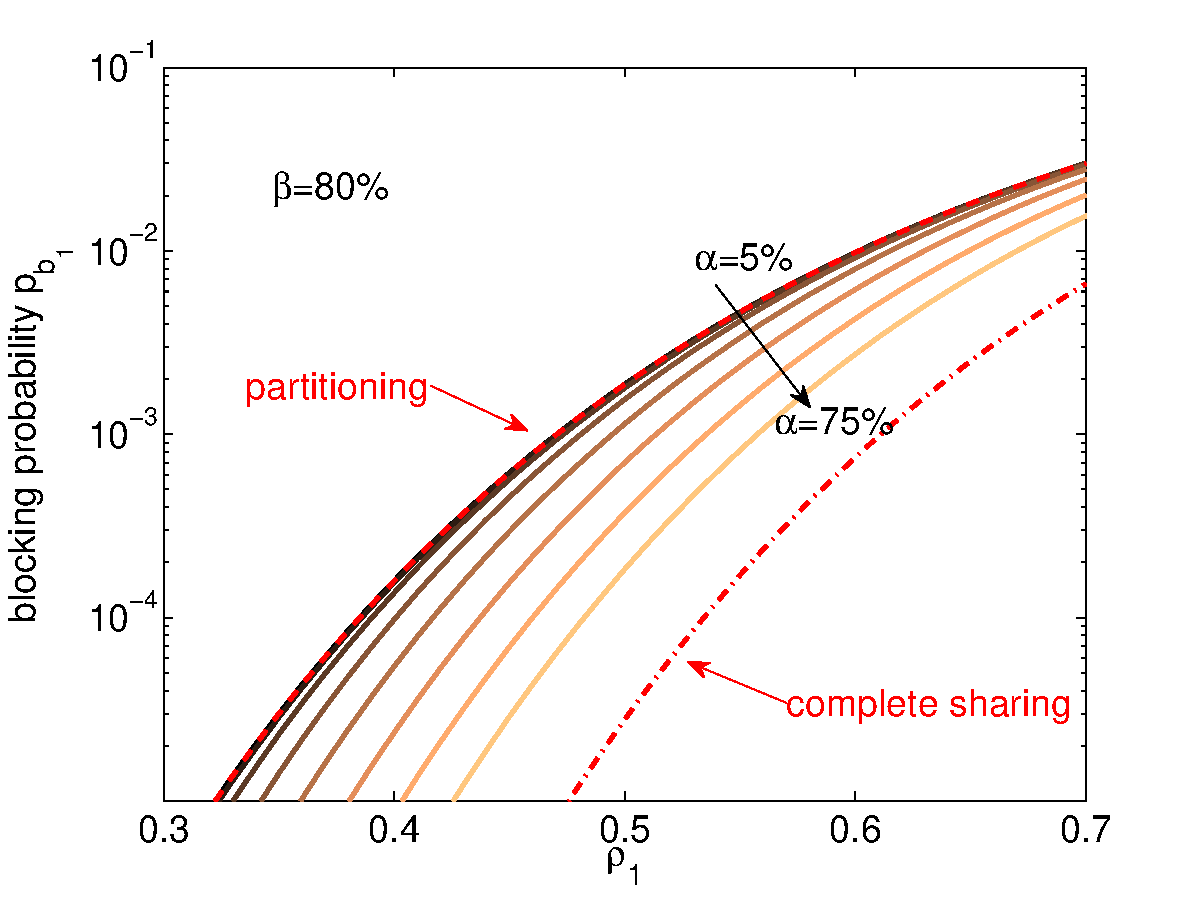
\includegraphics[width=\linewidth]{aggregation/performance_model/figures/m2_n20_alpha_equal}
 \caption{$\alpha$}
 \label{fig:m2_n20_alpha}
\end{subfigure}%
\begin{subfigure}{.49\textwidth}
 \centering
 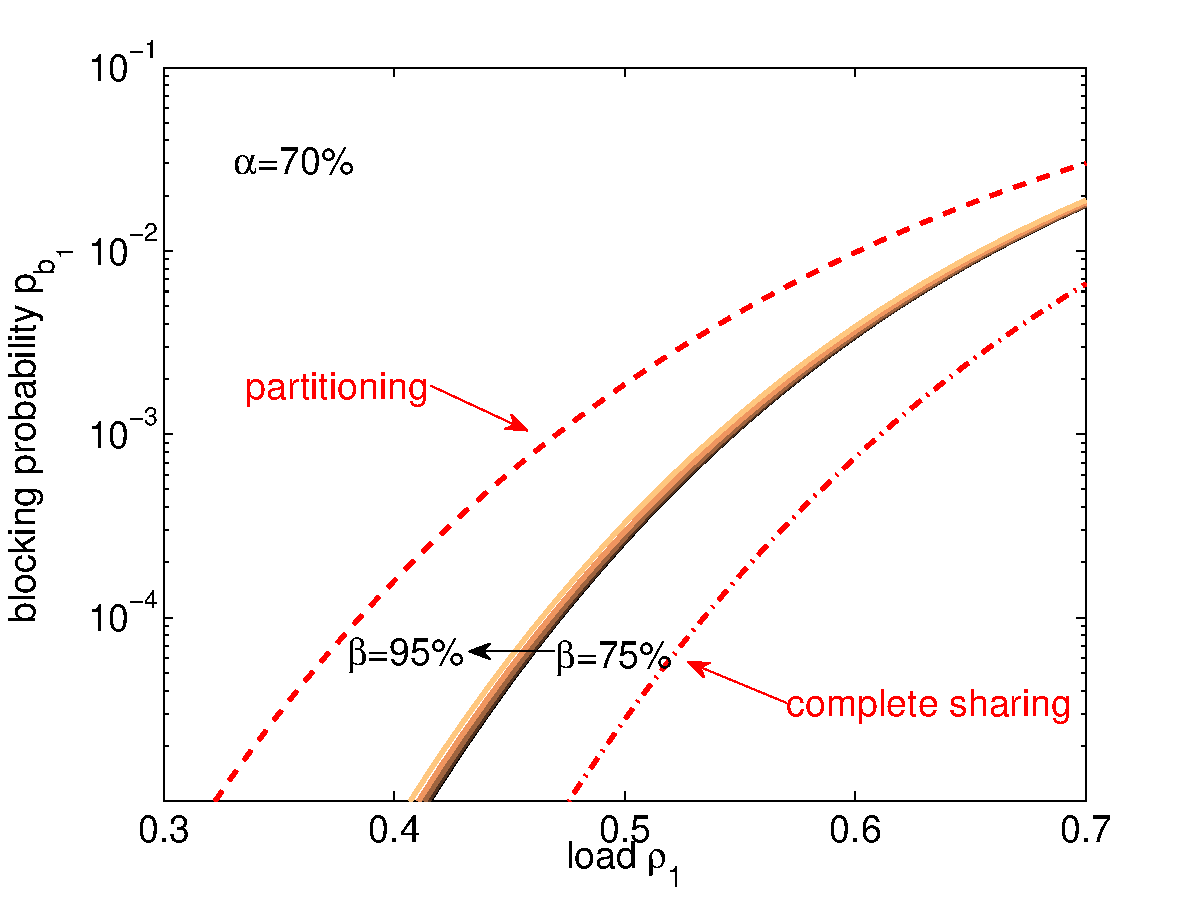
\includegraphics[width=\linewidth]{aggregation/performance_model/figures/m2_n20_beta_equal}
 \caption{$\beta$}
 \label{fig:m2_n20_beta}
\end{subfigure}
\begin{subfigure}{.49\textwidth}
 \centering
 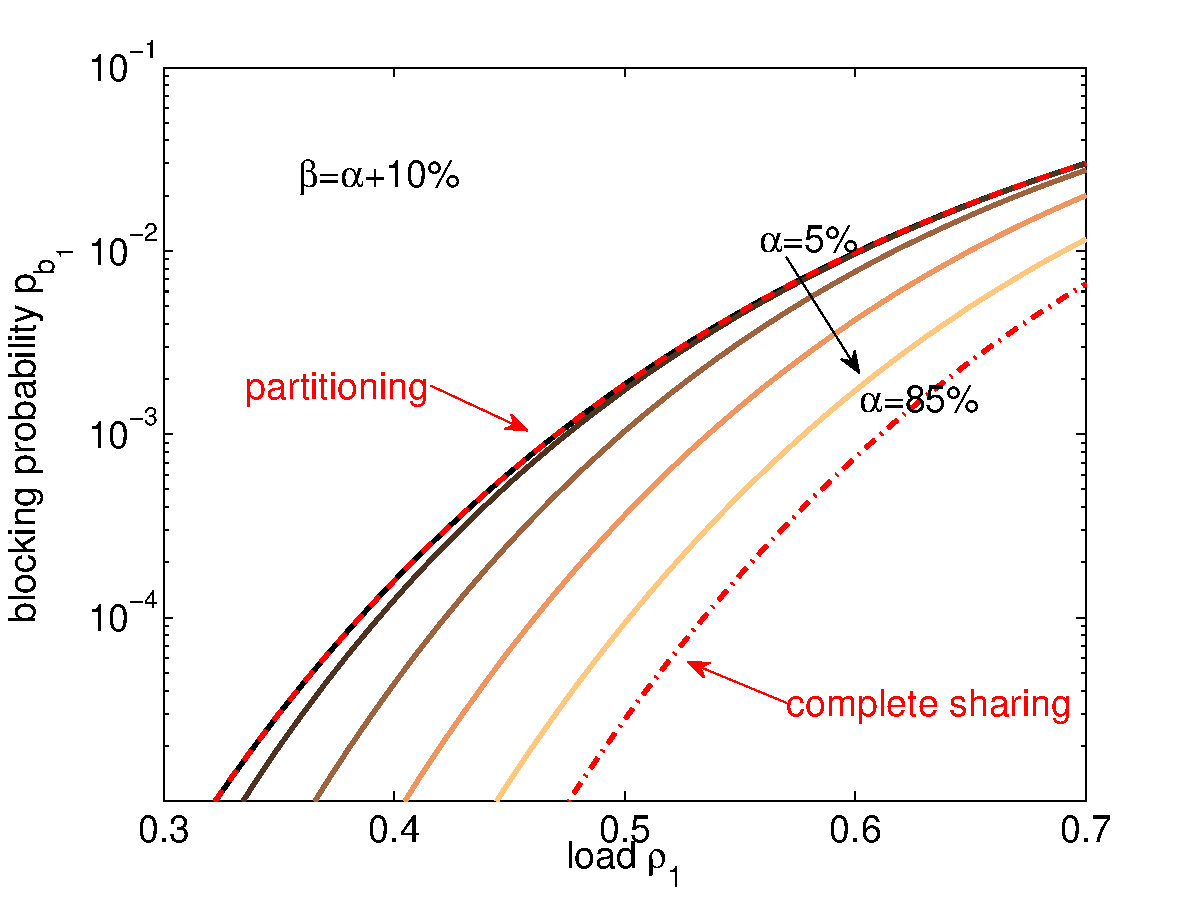
\includegraphics[width=\linewidth]{aggregation/performance_model/figures/m2_n20_alphaplus2_equal}
 \caption{$\alpha$ and $\beta$}
 \label{fig:m2_n20_alphaplus2_equal}
\end{subfigure}
\begin{subfigure}{.49\textwidth}
 \centering
 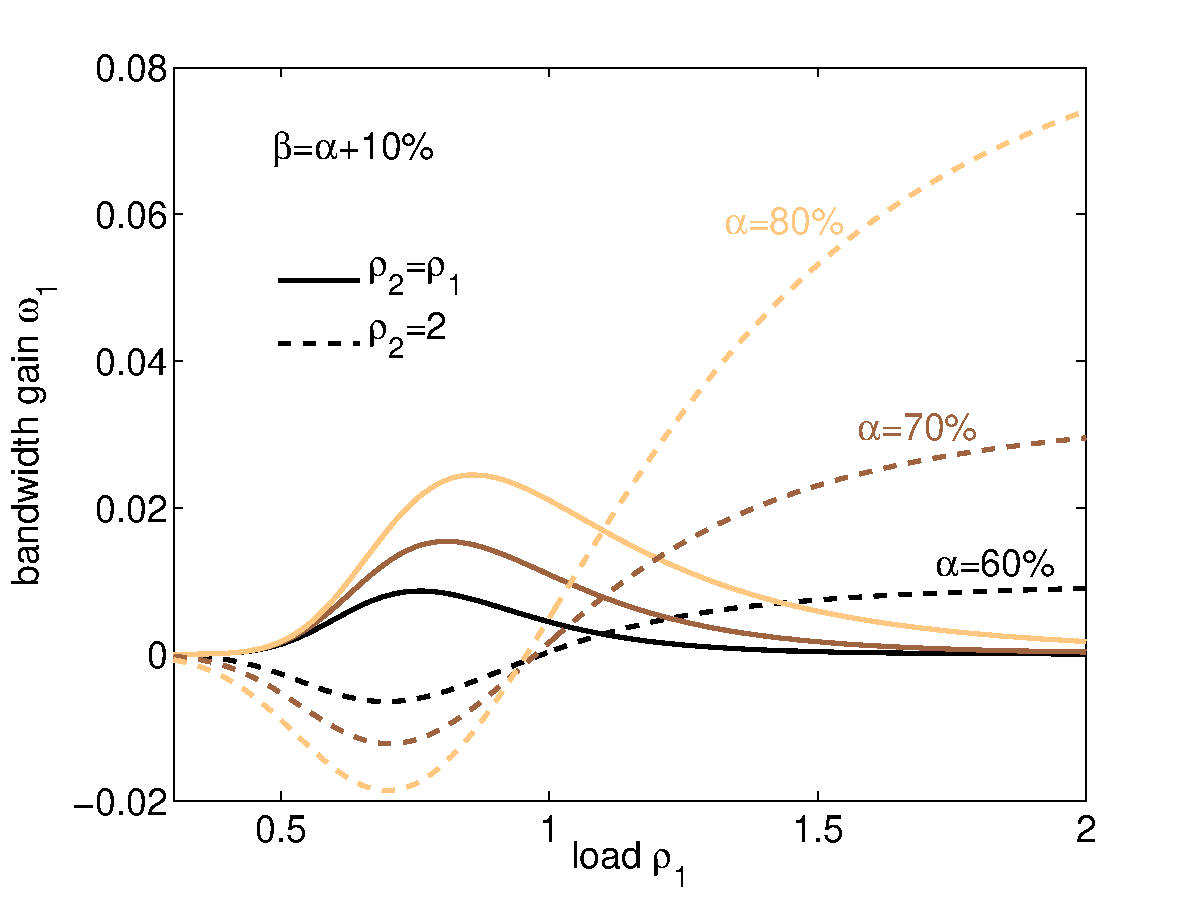
\includegraphics[width=\linewidth]{aggregation/performance_model/figures/bwgain_rhocomp}
 \caption{$\omega_1$}
 \label{fig:bwgain_rhocomp}
\end{subfigure}
\caption{Blocking probability $p_{b_1}$ dependent on thresholds (a) $\alpha$, (b) $\beta$ and (c) $\alpha$ and $\beta$, and (d) bandwidth gain $\omega_1$.}
\label{fig:m2_n20}
\end{figure}

% \begin{figure}[tb]
% 	\centering
% 	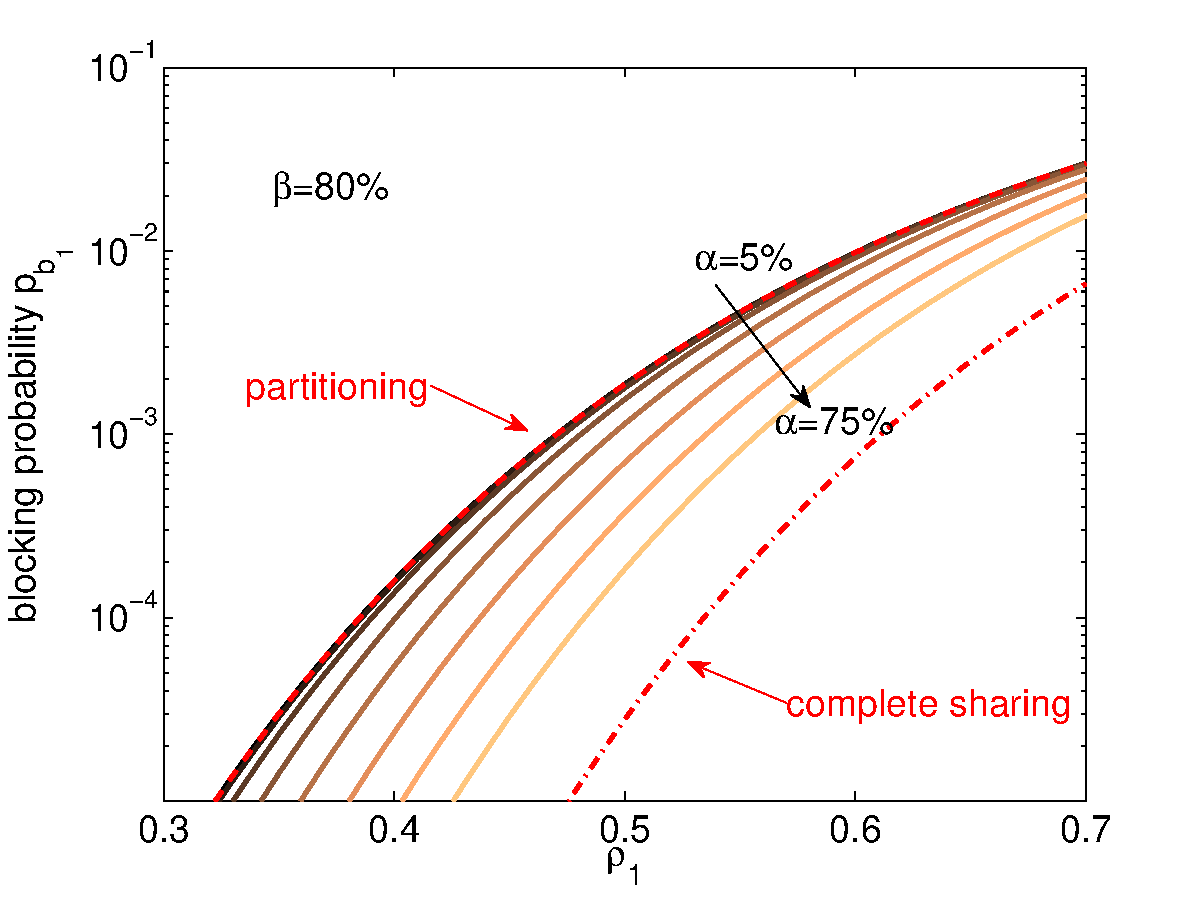
\includegraphics[width=0.5\textwidth]{aggregation/performance_model/figures/m2_n20_alpha_equal}
%  	\caption{Blocking probability of reference system dependent on threshold $\alpha$.}
%  	\label{fig:m2_n20_alpha}
% \end{figure}

Figure~\ref{fig:m2_n20_alpha} shows the blocking probability of the reference system $p_{b_1}$ dependent on the load $\rho_1$ for different support thresholds $\alpha$. The offloading threshold $\beta$ is constant at 80\% of the system capacity. For $\alpha=5\%$ a system only helps if it is empty and is not processing jobs. The systems work almost isolated from each other and thus the performance is equal to the performance of a single system. By increasing the support threshold $\alpha$ the systems can offer more help when one of the systems is overloaded and decrease the blocking probability. The support threshold $\alpha$ determines the amount of jobs that can be offloaded.

%\begin{figure}[tb]
%	\centering
% 	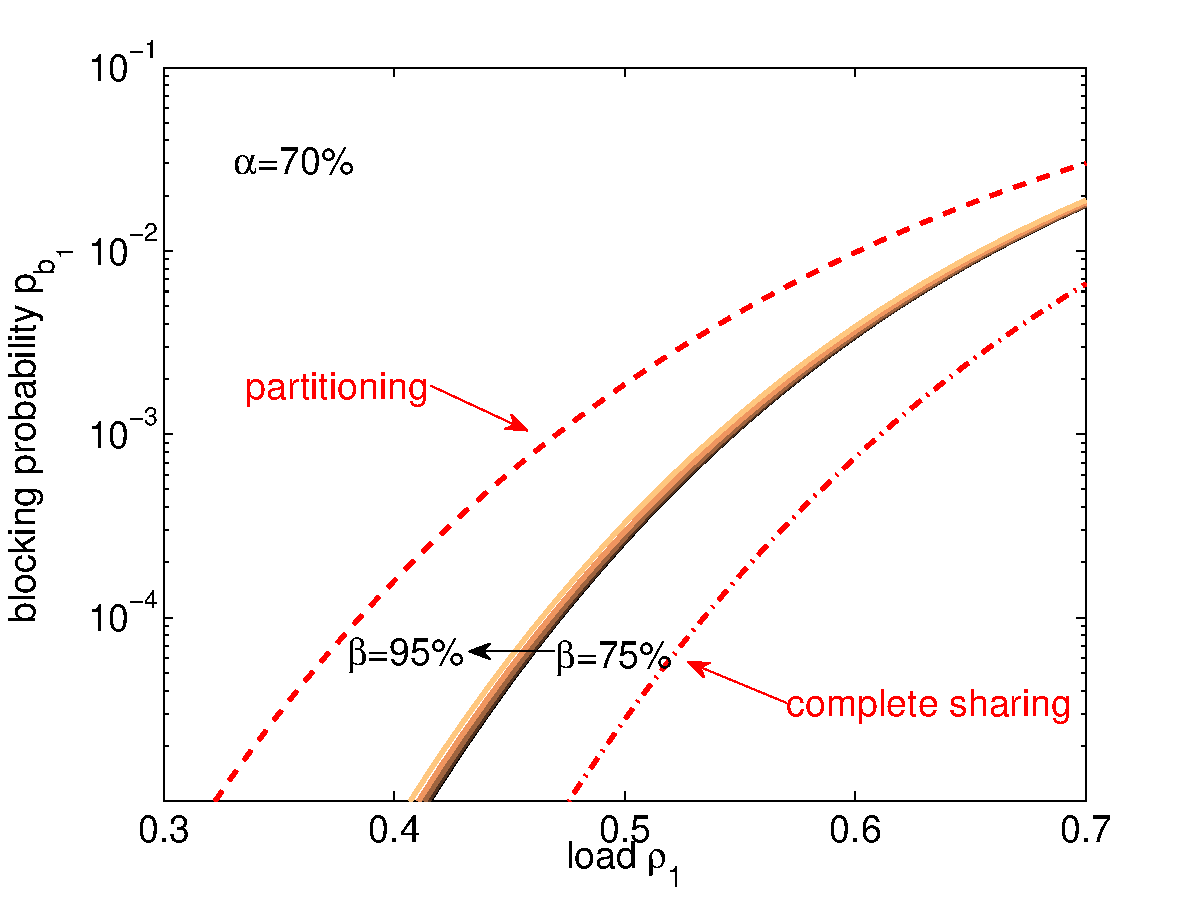
\includegraphics[width=0.5\textwidth]{aggregation/performance_model/figures/m2_n20_beta_equal}
%  	\caption{Blocking probability of reference system dependent on threshold $\beta$.}
%  	\label{fig:m2_n20_beta}
%\end{figure}

Figure~\ref{fig:m2_n20_beta} shows the blocking probability of the reference system $p_{b_1}$ dependent on the load $\rho_1$ for different offloading thresholds $\beta$. The support threshold $\alpha$ is constant at 70\% of the system capacity. The offloading threshold $\beta$ is increased from 75\% to 95\%. Increasing the offloading threshold has almost no impact on the blocking probability. The effect on the blocking probability is small, since the threshold $\beta$ just shifts the point of time at which the system starts offloading. The amount of jobs that can be offloaded is not dependent on $\beta$. The reason for the slight increase of the blocking probability with $\beta$ is that there are less chances to find the cooperating system in support state when $\beta$ is high.

%\begin{figure}[tb]
%	\centering
% 	\includegraphics[width=0.5\textwidth]{aggregation/performance_model/figures/m2_n20_alphaplusbeta}
%  	\caption{Blocking probability of reference system dependent on thresholds $\alpha$ and $\beta$.}
%  	\label{fig:m2_n20_alphaplusbeta}
%\end{figure}

We have seen that the performance of the system depends on the amount of jobs that can be offloaded, so the support threshold $\alpha$ needs to be set as high as possible. Theoretically, the support threshold could be set to the offloading threshold $\alpha=\beta$, so that a system would switch directly from support to offloading mode. However, in practice this may lead to problems, since the systems could switch unnecessarily frequently among the modes. This is especially the case if mode switches result in a high signalling overhead or imply expensive context switches. Therefore, a gap is left among the thresholds.
Hence, in order to prevent frequent mode switches, we set $\beta - \alpha$ to 10\%. In order to maximize the available bandwidth we can increase the support threshold $\alpha$.
%In the following we investigate the impact of that gap $\beta-\alpha$.
Figure~\ref{fig:m2_n20_alphaplus2_equal} shows the blocking probability of the reference system $p_{b_1}$ dependent on the load $\rho_1$ with fixed gap $\beta-\alpha$ for increasing support thresholds $\alpha$ from 5\% to 85\%. The blocking probability decreases with increasing $\alpha$, since more bandwidth fractions are shared among the systems.
However, the performance of the system can also drop if the support threshold $\alpha$ is to high, which can be seen in Figure~\ref{fig:bwgain_rhocomp}. Figure~\ref{fig:bwgain_rhocomp} shows the bandwidth gain $\omega_1$, c.f. Equ.~\ref{equ:gain}, of the reference system for an equally loaded cooperating system with $\rho_2=\rho_1$ and an overloaded cooperating system with $\rho_2=2$. If the cooperating system is equally loaded the bandwidth gain is always positive. If the cooperating system is overloaded, the bandwidth gain is negative, if the reference system is underutilized. In this case an increasing $\alpha$ has a negative effect on the bandwidth gain, because less bandwidth fractions are left for arrivals in the own system.
%With increasing gap $\alpha$ the number of shared bandwidth fractions is reduced, which increases the blocking probability. Hence, the best performance is achieved with a small gap.
%As stated above, frequent mode switches, due to fluctuations in the system load, can lead to performance problems.
To prevent the system from being overloaded, we leave 30\% of the capacity as buffer for peak periods and set the support threshold $\alpha$ to 70\%.
Hence, we set the support threshold $\alpha$ to 70\% and the offloading threshold $\beta$ to 80\% in the following.

% \subsubsection*{Equal Load}
%
% In this scenario, we assume that all access links are equal ($n=n_i, \forall i\in\{1,\ldots,m\}$), and face equal loads ($\lambda=\lambda_i, \forall i\in\{1,\ldots,m\}$) and policies ($\alpha = \alpha_i, \beta = \beta_i, \forall i\in\{1,\ldots,m\}$), according to Sec.~\ref{sec:equal}.
%
% Figure~\ref{fig:fp_bw_equ_m8} depicts the normalized received bandwidth $E[X_{A_1}]/n_1$ of the observed system depending on the load on each system for different numbers of cooperating systems $m$. The mean values with 95\% confidence intervals of 8 simulation runs are plotted for $m=8$ cooperating systems, as well as the received bandwidth in case of partitioning.
% The fixed point approximation fits the simulation results for $m=8$ cooperating systems.
% In any case the received bandwidth increases with the load on the systems.
% The systems can benefit only slightly from a higher number of cooperating systems, if the load on the systems approaches 1.
% In this case bandwidth fractions can be offloaded to temporarily underutilized systems, which increases the received bandwidth.
%
% However, the received bandwidth is only marginally higher than in the partitioning case.
% %This is highlighted considering the bandwidth gain $\omega_1$, which is depicted in Figure~\ref{fig:fp_bwgain_equ_m8} dependent on the load on the systems. In any case the bandwidth gain is less than 6\% with a maximum at $\rho\approx 0.79$.
% This depends on the fact that the load is shifted back an forth among the cooperating systems.
% A higher number of cooperating systems will not increase the bandwidth gain, since there is already a saturation effect for up to $m=8$ cooperating systems recognizable.
% %The bandwidth gain is never negative, which shows that under equal load at least no system suffers from the offloading mechanism.
